% Options for packages loaded elsewhere
% Options for packages loaded elsewhere
\PassOptionsToPackage{unicode}{hyperref}
\PassOptionsToPackage{hyphens}{url}
\PassOptionsToPackage{dvipsnames,svgnames,x11names}{xcolor}
%
\documentclass[
  letterpaper,
  DIV=11,
  numbers=noendperiod]{scrreprt}
\usepackage{xcolor}
\usepackage{amsmath,amssymb}
\setcounter{secnumdepth}{5}
\usepackage{iftex}
\ifPDFTeX
  \usepackage[T1]{fontenc}
  \usepackage[utf8]{inputenc}
  \usepackage{textcomp} % provide euro and other symbols
\else % if luatex or xetex
  \usepackage{unicode-math} % this also loads fontspec
  \defaultfontfeatures{Scale=MatchLowercase}
  \defaultfontfeatures[\rmfamily]{Ligatures=TeX,Scale=1}
\fi
\usepackage{lmodern}
\ifPDFTeX\else
  % xetex/luatex font selection
\fi
% Use upquote if available, for straight quotes in verbatim environments
\IfFileExists{upquote.sty}{\usepackage{upquote}}{}
\IfFileExists{microtype.sty}{% use microtype if available
  \usepackage[]{microtype}
  \UseMicrotypeSet[protrusion]{basicmath} % disable protrusion for tt fonts
}{}
\makeatletter
\@ifundefined{KOMAClassName}{% if non-KOMA class
  \IfFileExists{parskip.sty}{%
    \usepackage{parskip}
  }{% else
    \setlength{\parindent}{0pt}
    \setlength{\parskip}{6pt plus 2pt minus 1pt}}
}{% if KOMA class
  \KOMAoptions{parskip=half}}
\makeatother
% Make \paragraph and \subparagraph free-standing
\makeatletter
\ifx\paragraph\undefined\else
  \let\oldparagraph\paragraph
  \renewcommand{\paragraph}{
    \@ifstar
      \xxxParagraphStar
      \xxxParagraphNoStar
  }
  \newcommand{\xxxParagraphStar}[1]{\oldparagraph*{#1}\mbox{}}
  \newcommand{\xxxParagraphNoStar}[1]{\oldparagraph{#1}\mbox{}}
\fi
\ifx\subparagraph\undefined\else
  \let\oldsubparagraph\subparagraph
  \renewcommand{\subparagraph}{
    \@ifstar
      \xxxSubParagraphStar
      \xxxSubParagraphNoStar
  }
  \newcommand{\xxxSubParagraphStar}[1]{\oldsubparagraph*{#1}\mbox{}}
  \newcommand{\xxxSubParagraphNoStar}[1]{\oldsubparagraph{#1}\mbox{}}
\fi
\makeatother


\usepackage{longtable,booktabs,array}
\usepackage{calc} % for calculating minipage widths
% Correct order of tables after \paragraph or \subparagraph
\usepackage{etoolbox}
\makeatletter
\patchcmd\longtable{\par}{\if@noskipsec\mbox{}\fi\par}{}{}
\makeatother
% Allow footnotes in longtable head/foot
\IfFileExists{footnotehyper.sty}{\usepackage{footnotehyper}}{\usepackage{footnote}}
\makesavenoteenv{longtable}
\usepackage{graphicx}
\makeatletter
\newsavebox\pandoc@box
\newcommand*\pandocbounded[1]{% scales image to fit in text height/width
  \sbox\pandoc@box{#1}%
  \Gscale@div\@tempa{\textheight}{\dimexpr\ht\pandoc@box+\dp\pandoc@box\relax}%
  \Gscale@div\@tempb{\linewidth}{\wd\pandoc@box}%
  \ifdim\@tempb\p@<\@tempa\p@\let\@tempa\@tempb\fi% select the smaller of both
  \ifdim\@tempa\p@<\p@\scalebox{\@tempa}{\usebox\pandoc@box}%
  \else\usebox{\pandoc@box}%
  \fi%
}
% Set default figure placement to htbp
\def\fps@figure{htbp}
\makeatother





\setlength{\emergencystretch}{3em} % prevent overfull lines

\providecommand{\tightlist}{%
  \setlength{\itemsep}{0pt}\setlength{\parskip}{0pt}}



 


\KOMAoption{captions}{tableheading}
\makeatletter
\@ifpackageloaded{bookmark}{}{\usepackage{bookmark}}
\makeatother
\makeatletter
\@ifpackageloaded{caption}{}{\usepackage{caption}}
\AtBeginDocument{%
\ifdefined\contentsname
  \renewcommand*\contentsname{Table of contents}
\else
  \newcommand\contentsname{Table of contents}
\fi
\ifdefined\listfigurename
  \renewcommand*\listfigurename{List of Figures}
\else
  \newcommand\listfigurename{List of Figures}
\fi
\ifdefined\listtablename
  \renewcommand*\listtablename{List of Tables}
\else
  \newcommand\listtablename{List of Tables}
\fi
\ifdefined\figurename
  \renewcommand*\figurename{Figure}
\else
  \newcommand\figurename{Figure}
\fi
\ifdefined\tablename
  \renewcommand*\tablename{Table}
\else
  \newcommand\tablename{Table}
\fi
}
\@ifpackageloaded{float}{}{\usepackage{float}}
\floatstyle{ruled}
\@ifundefined{c@chapter}{\newfloat{codelisting}{h}{lop}}{\newfloat{codelisting}{h}{lop}[chapter]}
\floatname{codelisting}{Listing}
\newcommand*\listoflistings{\listof{codelisting}{List of Listings}}
\makeatother
\makeatletter
\makeatother
\makeatletter
\@ifpackageloaded{caption}{}{\usepackage{caption}}
\@ifpackageloaded{subcaption}{}{\usepackage{subcaption}}
\makeatother
\usepackage{bookmark}
\IfFileExists{xurl.sty}{\usepackage{xurl}}{} % add URL line breaks if available
\urlstyle{same}
\hypersetup{
  pdftitle={Muhammad Azikra Wira Pratama},
  pdfauthor={18224089 Muhammad Azikra Wira Pratama},
  colorlinks=true,
  linkcolor={blue},
  filecolor={Maroon},
  citecolor={Blue},
  urlcolor={Blue},
  pdfcreator={LaTeX via pandoc}}


\title{Muhammad Azikra Wira Pratama}
\usepackage{etoolbox}
\makeatletter
\providecommand{\subtitle}[1]{% add subtitle to \maketitle
  \apptocmd{\@title}{\par {\large #1 \par}}{}{}
}
\makeatother
\subtitle{Tugas Portofolio Komunikasi Interpersonal dan Publik}
\author{18224089 Muhammad Azikra Wira Pratama}
\date{2025-10-05}
\begin{document}
\maketitle

\renewcommand*\contentsname{Table of contents}
{
\hypersetup{linkcolor=}
\setcounter{tocdepth}{2}
\tableofcontents
}

\bookmarksetup{startatroot}

\chapter*{Hallo Semua}\label{hallo-semua}
\addcontentsline{toc}{chapter}{Hallo Semua}

\markboth{Hallo Semua}{Hallo Semua}

\begin{figure}[H]

{\centering \pandocbounded{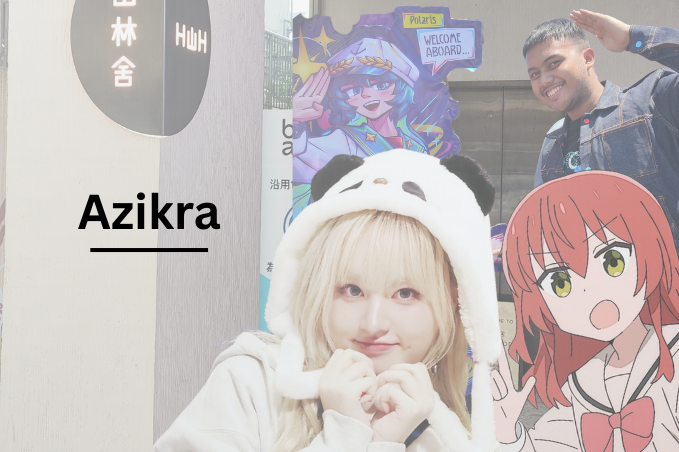
\includegraphics[keepaspectratio]{images/CoverIstri.png}}

}

\caption{Profil diri}

\end{figure}%

Muhammad Azikra Wira Pratama, yang akrab dipanggil ``Zik'' atau
``Zikra'', merupakan mahasiswa Sekolah Teknik Elektro dan Informatika --
Komputasi, Institut Teknologi Bandung (Angkatan 2024), dengan program
studi Sistem dan Teknologi Informasi (kode II).

Zikra lahir di Pekanbaru pada tahun 2006 dan saat ini berdomisili di
Cimahi.

\begin{center}\rule{0.5\linewidth}{0.5pt}\end{center}

\section*{Connect with Me}\label{connect-with-me}
\addcontentsline{toc}{section}{Connect with Me}

\markright{Connect with Me}

\begin{itemize}
\tightlist
\item
  Email :
  \href{mailto:18224089@std.stei.itb.ac.id}{\nolinkurl{18224089@std.stei.itb.ac.id}}
\end{itemize}

\bookmarksetup{startatroot}

\chapter{All About Me}\label{all-about-me}

\begin{center}\rule{0.5\linewidth}{0.5pt}\end{center}

\section{Identitas Diri}\label{identitas-diri}

\begin{longtable}[]{@{}ll@{}}
\toprule\noalign{}
\textbf{Nama} & Muhammad Azikra Wira Pratama \\
\midrule\noalign{}
\endhead
\bottomrule\noalign{}
\endlastfoot
\textbf{Program Studi} & Sistem dan Teknologi Informasi \\
\textbf{NIM} & 18224089 \\
\textbf{Tujuan} & Memperkenalkan sosok diri secara reflektif \\
\end{longtable}

\begin{center}\rule{0.5\linewidth}{0.5pt}\end{center}

\section{Refleksi Diri}\label{refleksi-diri}

Portofolio ini saya buat sebagai sarana untuk \textbf{merefleksikan diri
saya sebenarnya} bagaimana saya \textbf{memandang diri sendiri}, dan
bagaimana saya \textbf{menampilkan diri kepada orang lain}.\\
Melalui proses ini, saya berusaha untuk memahami siapa saya di balik
peran dan ekspektasi sosial yang saya jalani setiap hari.

Saya percaya bahwa dengan memahami diri secara jujur, saya dapat
\textbf{hidup dengan lebih autentik, selaras dengan nilai-nilai yang
saya yakini}, dan berinteraksi dengan orang lain secara lebih terbuka
dan bermakna.

\begin{center}\rule{0.5\linewidth}{0.5pt}\end{center}

\begin{quote}
\emph{``Hujan tidak selalu berarti sedih, kadang hanya cara dunia
mengingatkan kita untuk berhenti sejenak.''}
\end{quote}

\begin{center}\rule{0.5\linewidth}{0.5pt}\end{center}

\section{Siapa saya}\label{siapa-saya}

Kenalin saya \textbf{Muhammad Azikra Wira Pratama}, atau biasa dipanggil
\textbf{Zik/Zikra}. Saya mahasiswa dari program studi Sistem dan
Teknologi Informasi (II), Fakultas STEI, angkatan 2024.

Saya lahir di \textbf{Pekanbaru} dan kini tinggal di \textbf{Cimahi}.
Walau saya berdomisili Cimahi, saya sangat sering pergi ke
\textbf{Bandung}.

\begin{center}\rule{0.5\linewidth}{0.5pt}\end{center}

\section{Apa yang Membentuk Saya}\label{apa-yang-membentuk-saya}

Sejak kecil, saya selalu tertarik dengan bidang teknologi yang dimulai
dari kesukaan saya ketika memainkan gim. Bidang ini saya telusuri
sedikit-sedikit hingga jadi tertarik untuk masuk ke jurusan di dunia
informatika. Kampus yang saya impikan itu \textbf{ITB} dan ketika
mengetahui bahwa terdapat fakultas \textbf{STEI} saya menjadikan hal
tersebut target selama menempuh pendidikan \textbf{SMA}.

\begin{center}\rule{0.5\linewidth}{0.5pt}\end{center}

\section{Bagaimana Saya Melihat Diri}\label{bagaimana-saya-melihat-diri}

Saya orang yang \textbf{pendiam di awal}, tapi \textbf{kalau sudah
nyaman akan sangat ekpresif}. Saya cenderung memilih diam jika ada
diberikan waktu untuk berpikir dalam memutuskan suatu hal.

Hal kecil yang terjadi kadang saya perhatikan seperti apa respons
spontan yang diberikan ketika saya berbicara, bertindak, atau bercanda.
Saya berusaha untuk memerhatikan diri agar tidak menyinggung perasaan
orang. Hal tersebutlah yang membuat saya belajar mengenai
\textbf{Komunikasi diri}, tentang bagaimana jujur tanpa harus membuka
hal pribadi.

\begin{center}\rule{0.5\linewidth}{0.5pt}\end{center}

\section{Sisi Ringan Saya}\label{sisi-ringan-saya}

Mengenai hal tadi selain memerhatikan hal kecil dari diri saya, kadang
saya memerhatikan juga aktivitas unik dari orang di sekitar saya
terutama teman-teman saya.

Hal ini sering saya jadikan seperti upaya saya untuk menjadi lebih dekat
dan terhubung dengan mereka. Saya bisa menggunakan teknik tersebut
dengan pembicaraan ringan, bercanda, dan hal menarik lainnya.

Selain kebiasaan tersebut dalam lingkup sosial, ketika sedang bersantai
sendiri saya sering mendengarkan lagu tenang atau sedih. Saya cenderung
menyelam dalam perasaan sendiri untuk refleksi atau sekedar istirahat
dari lingkup sosial.

\begin{center}\rule{0.5\linewidth}{0.5pt}\end{center}

\section{Refleksi dan Nilai Hidup}\label{refleksi-dan-nilai-hidup}

Bagi saya, \textbf{komunikasi diri} adalah tentang keberanian untuk
jujur pada diri sendiri. Saya belajar bahwa \textbf{menerima kelemahan
bukan tanda menyerah}, tapi langkah pertama untuk tumbuh.

Saya ingin hidup dengan prinsip:

\begin{quote}
\emph{``Tidak harus selalu benar, tapi harus selalu mau belajar.''}
\end{quote}

Dengan memahami diri, saya berharap bisa \textbf{lebih autentik,
konsisten dengan nilai yang saya yakini}, dan membawa empati ke setiap
hubungan dalam kehidupan.

\begin{center}\rule{0.5\linewidth}{0.5pt}\end{center}

\section{Penutup}\label{penutup}

Portofolio ini bukan hanya tentang siapa saya sekarang, tapi juga
tentang siapa saya ingin jadi.\\
Mungkin hujan akan tetap turun, tapi selama saya melangkah dengan jujur,
saya tahu matahari akan muncul pada waktunya.

\bookmarksetup{startatroot}

\chapter{My Songs for You}\label{my-songs-for-you}

\begin{center}\rule{0.5\linewidth}{0.5pt}\end{center}

Ini adalah lagu yang sangat berarti bagi saya.

\url{https://www.youtube.com/watch?v=HwGFMez_Tnc}

Lagu ini menemani saya yang sedang mengalami banyaknya masalah, di akhir
jenjang SMA. Liriknya menggambarkan dimana banyak kenyataan pahit yang
terjadi, dunia akan terus berjalan seperti hujan yang akan selalu turun
kapanpun itu. Apapun yang terjadi dalam kehidupan, harus selalu maju
karena hujan tidak akan berhenti walaupun saat seseorang tenggelam dalam
kesedihan.

Why am I singing for you? \href{./Rivers\%20In\%20My\%20Mind.mp3}{River
in my Mind}

Falling in love everyday \href{./Heaven\%20on\%20Earth.mp3}{Heaven on
Earth}

\bookmarksetup{startatroot}

\chapter{My Stories for You}\label{my-stories-for-you}

A story about my oldest daughter
\href{https://azrl.wordpress.com/2020/07/18/gaun-pengantin-gladys/\#comment-28004}{Gaun
Pemngantin Gladys}

A message to my daughter
\href{https://azrl.wordpress.com/2021/10/06/the-child-who-learned-to-walk-at-the-disneyland/}{The
Child Who Learned to Walk at the Disneyland}

A story for my students
\href{https://azrl.wordpress.com/2008/04/21/fly-my-eagle-fly/}{Fly Eagle
Fly}

A (true) story for my teachers
\href{\%3Chttps://azrl.wordpress.com/2012/11/28/perginya-sang-mahaputera-dan-mahaguru-berkemeja-putih/}{Sang
Mahaguru, Sang Mahaputera}

Teasing story \url{https://www.youtube.com/watch?v=Dg_4PbBlBf4}

\bookmarksetup{startatroot}

\chapter{My Shapes}\label{my-shapes}

\bookmarksetup{startatroot}

\chapter{My Personal Reviews}\label{my-personal-reviews}

Berikut cara saya melakukan review
\href{./Doc.5.Mengevaluasi-Esai-Berdasarkan-Rubrik.pdf}{Menilai dan
Mengevaluasi Esai Berdasarkan Rubrik}

\bookmarksetup{startatroot}

\chapter{My Concepts}\label{my-concepts}

Mau hidup epik ? \href{lifestory.pdf}{Write your Life Story}

Apa itu berkonsep?

\url{https://youtu.be/QVfUlVBO80U?si=yM6q_rwV9rcDBbu7}

\bookmarksetup{startatroot}

\chapter{My Opinions}\label{my-opinions}

SApa itu beropini? \href{BM\%20Opini.mp4}{Opini Berpengaruh}

Bagiamana menjaadi menarik? \href{./Interesting.mp4}{Menjadi Menarik}

\bookmarksetup{startatroot}

\chapter{My Innovations}\label{my-innovations}

\bookmarksetup{startatroot}

\chapter{My Knowledge}\label{my-knowledge}

Cara saya mengkomunikasikan sebuah pengatahuan sebagai petunjuk bagi
orang lain 1) saya tulis
\href{Rekomendasi\%20Presentasi\%20Efektif(Contoh\%20Makalah).pdf}{makalah
sebagai bahan utama} 2) lalu saya buat
\href{Contoh\%20Transkrip\%20Presentasi.pdf}{transkrip ucapan lisan} 3)
kemudian saya kembangkan
\href{Rekomendasi\%20Presentasi\%20(Contoh\%20Slides).pdf}{slide
pendukung trnsskrip} 4) lalu saya memproduksivideo audio visual
\url{https://youtu.be/ZbghfMvnPZc} \url{https://youtu.be/ZbghfMvnPZc}

\bookmarksetup{startatroot}

\chapter{My Professional Reviews}\label{my-professional-reviews}

Untuk melkukan review, seperti pada
\href{../My_Personal_Reviews/Doc.5.Mengevaluasi-Esai-Berdasarkan-Rubrik.pdf}{pendekatan
AI}, kita membutuhkan rubrik - Rubrik
\href{Dok.4.a.Rubrik_Kisah.pdf}{Kisah} - Rubrik
\href{Dok.4.b.Rubrik_Konsep.pdf}{Konsep} - Rubrik
\href{Dok.4.c.Rubrik_Opini.pdf}{Opini}

\bookmarksetup{startatroot}

\chapter{Summary}\label{summary}

In summary, this book has no content whatsoever.

\bookmarksetup{startatroot}

\chapter*{References}\label{references}
\addcontentsline{toc}{chapter}{References}

\markboth{References}{References}

\phantomsection\label{refs}




\end{document}
